% !Mode:: "TeX:UTF-8"
%%==========================
%% chapter01.tex for SJTU Master Thesis
%% based on CASthesis
%% modified by wei.jianwen@gmail.com
%% version: 0.3a
%% Encoding: UTF-8
%% last update: Dec 5th, 2010
%%==================================================

%\bibliographystyle{sjtu2} %[此处用于每章都生产参考文献]
\chapter{基于隐式衣服属性变量的姿势预测}
\label{chap:model}

\begin{figure}[tbp]
\centering
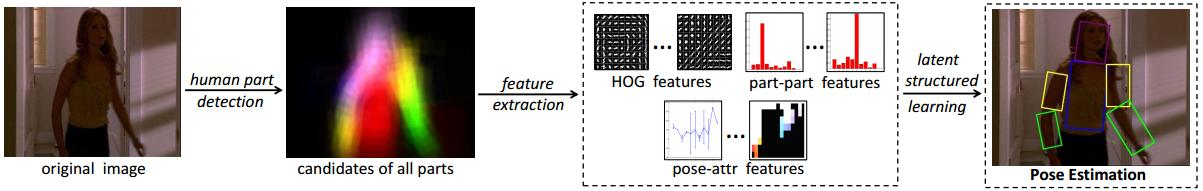
\includegraphics[width=\textwidth]{img/frame.pdf}
\caption{ \textbf{我们算法的框架} }
\label{fig:frame}
\end{figure}

在图\ref{fig:frame}中,我们描述了我们提出的方法。
首先,我们进行一步预处理,检测出图片中可能的人体姿势,构成一个人体姿势解的候选集。
这使得我们可以对搜索空间进行管理,从而降低我们的搜索空间,加速我们的求解过程。
其次,我们设计并抽取了人体部位和衣服属性相关的特征。
接着,我们采用隐变量结构式支持向量机框架进行模型参数的学习,
最后,我们设计了一个高效的预测算法来求得人体部位和衣服属性的近似最优解。
需要注意的是,我们的方法最后也给出了一个精确的衣服属性类别,这样可以将具有相似衣服属性的图片聚集在一起。
这也是我们有贡献的一步。


\begin{table}
\label{tb:attr}
\centering
\caption{人体躯干和衣服属性的关系}
\begin{tabular}{|c|c|c|c|} \hline
衣服属性& 人体部位& 底层特征& 类别数目\\ \hline
Sleeve &  All arms & Color Histogram & 3 \\ \hline
Neckline & Torso + Head & HOG & 4\\ \hline
 Pattern & Torso & LBP~\cite{lbp} & 5\\ \hline
\end{tabular}
\end{table}

在介绍我们的模型细节之前,我们介绍一些本文中需要用到的符号表示。
我们用$I$来表示一副图片,用一个矩形框$(x, y, s, \theta)$ 来表示一个人体部位,
$(x, y)$是人体部位的坐标,$s$是大小,$\theta$是人体部位的倾斜度。
假设我们一副图片中有$m$个人体部位(在本文中,$m = 6$)。
为了使模型输入的搜索空间在一个可控的范围内,我们采用目前结果最好的方法为每个人体部位产生40个候选解。因此我们问题的输入空间可以表示为:
\begin{equation}
    \mathcal{X} = \left\{ \mathbf{x}|\mathbf{x} = ( \mathbf{b}_1, \mathbf{b}_2, \cdots, \mathbf{b}_m ) \right\},
\end{equation}

对于一个图片$\mathbf{x}$,$\mathbf{b}_i$表示第i个人体部位的候选解集(包含40个候选解)。
而我们人体姿势的输出空间为:
\begin{equation}
    \mathcal{P} = \{\mathbf{p}| \mathbf{p}=(p_1,p_2,\cdots,p_m), \forall i, 1\leq p_i \leq 40\},
\end{equation}
$p_i$ 是一个下标,它表示候选解集$\mathbf{b}_i$中第i个元素的下标。

我们的目的是将衣服属性加入到人体姿势预测问题中,
通过捕捉到人体部位与衣服属性之间的关系。
在本文中,我们考虑了三种衣服属性,包括Neckline(衣领样式)、Pattern(衣服纹理)和Sleeve(袖子)。
对于每一个衣服属性来说,它会有多个样式,比如袖子属性有长袖、短袖和无袖等。
在表\ref{tb:attr}中,我们对于每一个衣服属性,根据经验定义了它的类别数。
因此我们问题中衣服属性的输出空间为:
\begin{equation}
    \mathcal{A} = \left\{ \mathbf{a}|\mathbf{a} = (a_1, a_2, \cdots, a_n), \forall r, 1 \leq a_r \leq T_r \right\}.
\end{equation}

$n$ 是衣服属性的个数(本文中,$n = 3$),$a_r$ 是第$r$个属性的类别标签。
需要注意的是,我们并不知道这些属性的类别标签的具体含义,比如$a_1 = 1$可能代表短袖,也可能代表长袖。
因为在本文中,识别衣服属性是一个聚类问题,我们只把具有相似衣服属性类别的图片样本聚集到一起。

因此我们的问题(基于隐变量衣服属性的人体姿势预测)可以形式化为一下式子:
\begin{equation}
    f: \mathcal{X} \rightarrow \mathcal{Y},
    \label{eq:task_func}
\end{equation}
其中 $\mathcal{Y}$ 是我们问题的输出空间,它被定义如下:
\begin{equation}
    \mathcal{Y} = \left\{ \mathbf{y}|\mathbf{y} = (\mathbf{p},\mathbf{a}), \mathbf{p} \in \mathcal{P}, \mathbf{a} \in \mathcal{A} \right\},
\end{equation}

考虑预测函数 $f$,我们假定有一个分数函数 $S$ 定义了输入-输出对 $(\mathbf{x}, \mathbf{y})$ 的匹配程度:
\begin{equation}
\label{eq:map}
    S(\mathbf{x}, \mathbf{y};\beta) = \langle \beta, J(\mathbf{x}, \mathbf{y}) \rangle
\end{equation}

其中 $\langle \cdot \rangle$ 表示两个向量的内积,
$J(\cdot, \cdot)$ 是我们问题的联合特征表示,
$\beta$ 是需要去学习的模型参数。

因此,我们的匹配函数 $f$ 可以写为如下表示:
\begin{equation}
    f(\mathbf{x}; \mathbf{\beta}) = arg \max_{ \mathbf{y} \in \mathcal{Y} } S(\mathbf{x}, \mathbf{y}; \mathbf{\beta})
    %f(\mathbf{x}; \mathbf{\beta}) = \argmax { \mathbf{y} \in \mathcal{Y} } S(\mathbf{x}, \mathbf{y}; \mathbf{\beta})
    \label{eq:score}
\end{equation}
这是一个包含隐变量的结构式学习问题,其中衣服属性是隐变量。
我们模型的学习过程是来自于\cite{dpm}这篇文章的启发,是一个不断调整的策略,来提升隐变量的预测精度。


在本章中,我们将描述我们提出的模型,这是一个典型的结构式学习(structure learning)问题。
我们将分为三部分来描述我们的模型。
第一部分是联合特征的分析与设计,这是所有结构式学习问题中很关键的一步,因为设计好了特征,才有可能使得我们的模型达到一个比较好的结果。
我们设计的特征既包含了人体部位的特征,也包含了人体部位与衣服属性的联合特征,这样我们将衣服属性的特征很好的结合到传统的人体姿势预测问题中。
第二部分是基于隐变量的结构式学习,这是我们模型的参数学习过程。
其中包含了多个问题的解决方案,包括隐变量的初始化,负样本空间的管理,以及模型训练的策略问题。
模型参数的学习也要用到第三部分的预测算法,因为模型训练过程中,需要调用预测算法来估计局部最优解,进而得到正样本。
第三部分是基于模型的有环图预测算法,这部分的输入是训练好的模型和一张新的测试图片,输出是人体姿势和衣服属性的最优解。
下面我们详细介绍每一部分。

\section{联合特征分析与设计}
联合特征的设计是所有结构式学习中比较关键的一步\cite{svm-struct},特征设计的好坏关系到模型预测能力的好坏,并决定了模型预测能力的上限。
我们设计了两类特征来构成我们问题的联合特征$J(\mathbf{x}, \mathbf{y})$,包括人体姿势相关的特征$j_p(\mathbf{x}, \mathbf{p})$,以及人体姿势和衣服属性相关的特征$j_{pa}(\mathbf{x}, \mathbf{y});$。

总体来看,我们问题的联合特征表示如下:
\begin{equation}
    \label{eq:feature}
    \langle \mathbf{\beta}, J(\mathbf{x},\mathbf{y}) \rangle = \langle \mathbf{\beta}_p, j_p(\mathbf{x}, \mathbf{p}) \rangle + \langle \mathbf{\beta}_{pa}, j_{pa}(\mathbf{x},\mathbf{y}) \rangle
\end{equation}
下面,我们详细介绍我们是如何设计每一类特征的。




\begin{algorithm}
\caption{包含隐变量的结构式支持向量机学习}
\begin{algorithmic}[1]
    \REQUIRE 正例样本集合, 负例样本集合, 初始模型参数 $\beta$, 重调整策略的次数 $t_1$, 困难负例挖掘的迭代次数 $t_2$.
    \ENSURE 最终模型 ${\beta}^*$.
    \STATE 初始化最终模型: ${\beta}^* = \beta$.
    \STATE 标记负例集为 $F_n = \emptyset$.
    \FOR{ relabel = 1 to $t_1$ }
        \STATE 标记正例集为 $F_p = \emptyset$.
        \STATE 将正例逐个加入 $F_p$.
        \FOR{ iter = 1 to $t_2$ }
            \STATE 将负例逐个加入 $F_n$.
            \STATE ${\beta}^* := \mathrm{Pegasos}({\beta}^*, F_p \bigcup F_n)$.\\
            \STATE 将容易的负例去除掉: \\
             删除掉那些负例特征 $v$ 满足 $\langle{\beta}^*, v \rangle < -1$ from $F_n$.
        \ENDFOR
    \ENDFOR
\end{algorithmic}
\label{alg:train}
\end{algorithm}


\subsection{人体躯干相关特征}
对于一个输入样本$\mathbf{x}$,我们用方向梯度直图(HOG)\cite{hog} 来描述一个候选解的形状,
而且我们考虑了两个相连的人体躯干之间的形变约束关系:
\begin{equation}
    j_p(\mathbf{x}, \mathbf{p}) = \sum_{i=1}^m hog(\mathbf{x}, p_i) + \sum_{(i, j) \in E_p} d(\mathbf{x}, p_i, p_j),
\end{equation}
其中$E_p$ 是相连人体躯干的集合。

形变特征的设计主要考虑相连人体躯干之间的几何约束,包括相对位置、相对角度和两者的距离,计算公式为:
$[x_j - x_i, y_j - y_i, (x_j - x_i)^2, (y_j - y_i)^2]$~\cite{deva11}.

\subsection{衣服属性相关特征}
通过衣服属性特征,我们将衣服属性结合到我们模型当中。
需要注意的是,一个衣服属性可能会关联多个人体躯干,比如袖子会关联到所有的手臂躯干。
对于一个给定的属性 $r$,我们用 $r_p$ 来表示跟属性 $r$ 相关的人体躯干,用 $P_r$ 来表示这种对应关系的配置信息。
在表 \ref{tb:attr} 的第二栏中,我们给出了衣服属性和人体躯干之间的对应关系。
显而易见,对于不同的衣服属性,应该使用不同的底层特征来描述,这样才能达到很好的特性 \cite{clothliu}。
我们在表 \ref{tb:attr} 的第三栏给出了这种对应关系,每种衣服属性对应的底层特征。

因此衣服属性特征可以形式化为:
\begin{equation}
    \label{eq:j_pa}
    j_{pa}(\mathbf{x}, \mathbf{y}) = \sum_{r=1}^n \Psi(\mathbf{x}, P_r, a_r)
\end{equation}
其中 $\Psi(\mathbf{x}, P_r, a_r)$ 表示从样本 $x$ 中抽取出来的关于 人体躯干的对应配置 $P_r$ 和衣服属性类别 $a_r$ 的衣服属性特征。


跟之前的工作\cite{shen2014unified}类似,我们将衣服属性特征设计为底层特征和属性类别向量的外积,这样可以采用一种简单有效的方式将人体躯干和衣服属性联合起来。
首先,我们将衣服属性的类别标签 $a_r$ 转化为一个维度是 $T_r$ 的向量 $L(a_r)$,
在这个向量里,只有一维数据是1,其余都是0。
根据表 \ref{tb:attr},第$r$个衣服属性的底层特征依赖于下述两方面:
衣服属性对应的人体躯干和衣服属性标签。
我们用$F_r(P_r)$来表示第$r$个衣服属性对应的特征,并且跟衣服属性对应的人体躯干配置 $P_r$ 有关。

因此,我们的衣服属性特征 $\Psi(\mathbf{x}, P_r, a_r)$ 可以表示为以下式子:
\begin{equation}
    \Psi_{pa}(\mathbf{x}, P_r, a_r) = F_r(P_r) \otimes L(a_r)
\end{equation}
其中的符号操作 ``$\otimes$'' 表示将两个向量的外积之后的矩阵向量化。

\section{基于隐变量的结构式学习}
在上节中,我们设计了问题的联合特征,现在我们来考虑模型的训练问题。
我们的训练数据集有人体姿势的标签信息,这是人体姿势预测问题的所有标准数据集都拥有的数据信息。
但是数据集中没有衣服属性的标签信息,我们通过把衣服属性作为隐变量的方法去训练模型。

在本节中,我们提出了一个框架用来初始化这个结构式问题和学习所有的参数。
我们将问题的参数学习部分转化为一个LSSVM(Latent Structure Support Vector Machine,隐变量结构式支持向量机)训练问题来进行求解。
对于一个LSSVM问题,我们设计了一种重标记的方式来求解,并且结合数据挖掘(困难数据挖掘)技术来控制负样本空间的大小,
并且我们采用Pegasos\cite{pegasos}算法来进行在线学习,这样就可以解决因为负例空间巨大而造成的训练时间复杂度很大。

\begin{algorithm}
\caption{衣服属性预测算法}
\begin{algorithmic}[1]
    \REQUIRE 测试图片样本 $\mathbf{x}$, 模型参数 $\beta$ , 人体姿势的局部最优解 $\mathbf{p}$
    \ENSURE 衣服属性的最优解 $\mathbf{a^*}$
    \STATE 用 $T_r$ 来标记第 $r$-th 个衣服属性的种类数量
    \FOR {r:= 1 \textbf{to} 3}
        \STATE 选择使得下列分值函数值最高的衣服属性类型:\\
            %$\mathbf{a}_r = \argmax_{1 \leq r \leq T_r} \langle \beta_{pa}^r, j_{pa}(\mathbf{x}, P_r, a_r) \rangle $
            $\mathbf{a}_r = arg \max_{1 \leq r \leq T_r} \langle \beta_{pa}^r, j_{pa}(\mathbf{x}, P_r, a_r) \rangle $
    \ENDFOR
\end{algorithmic}
\label{alg:attr}
\end{algorithm}


\subsection{目标函数}
在这一小节中,我们需要定义问题的目标函数,即就是问题的优化函数,通过对优化函数的训练而求得我们最终的解。
而我们的优化函数目标是学习我们在式\ref{eq:map}中定义的匹配函数 $S(\mathbf{x}, \mathbf{y}; \beta)$,它将在后面联合估计预测中用到。
给定一个正例训样样本 $(\mathbf{x}, \mathbf{y})$,我们期望匹配函数 $S(\mathbf{x}, \mathbf{y}; \beta) \geq 1$。
另一方面,如果一个训练样本是负例,那么匹配函数的输出应该是小于$-1$的。
因此,给定一个训练集 $D = \{ (\mathbf{x}_1, \mathbf{y}_1, z_1), \cdots, (\mathbf{x}_q, \mathbf{y}_q, z_q) \}$, 其中 $z_k \in \{1, -1\}$ 表示第 $k$ 个样本是正例还是负例,我们可以通过优化以下函数来求解模型的参数 $\beta$:
\begin{equation}
\begin{split}
\min_{\beta}  \frac{1}{2} \|\beta\|^2 + C \sum_{k=1}^{q}\max(0, 1 - z_k S(\mathbf{x}_k, \mathbf{y}_k; \beta)).
    \label{eq:latent}
\end{split}
\end{equation}

\subsection{隐变量初始化}
对于一个包含隐变量的结构式学习问题,隐变量的初始化是关键的一个步骤。
在本问题中,衣服属性是作为隐变量的,而人体躯干对于我们来说是观察量,是有标签信息的。
为了模型的初始化,我们采用一种重标记的策略来更新正例中衣服属性的标签信息和模型参数$\beta$。

有很多种方式可以进行模型中隐变量的初始化,我们可以随机的为隐变量设定标签信息,但是很有可能造成模型的不稳定性。
在本文中,我们首先根据人体躯干的标签信息抽取每个衣服属性对应的底层特征,
然后采用$k$-Means聚类算法来获得每个衣服属性的类中心,
其中 $K$ 是我们在表\ref{tb:attr}中定义的衣服属性的类别数目。
因此,隐变量衣服属性的初始标签可以通过其最近的类中心来决定。
通过这种初始化的方式,我们得到了所有衣服属性的初始标签信息,所以我们可以求解问题 \eqref{eq:latent} 来得到初始的模型参数 $\beta$。

\subsection{模型训练策略}
由于初始化的衣服属性类别信息不够精确,我们采用一种重标记的策略来不断更新衣服属性值。
即就是,当给定了模型的参数 $\beta$ 和人体躯干的标签信息后,我们通过最大化匹配函数 $S(\mathbf{x}, \mathbf{y}; \beta)$ 来预测衣服属性的标签信息,计算细节在算法 \ref{alg:attr} 中。
需要注意的是,根据我们联合特征的设计规则来看,衣服属性的预测与人体躯干的特征无关的,它只与衣服属性特征有关。

根据公式\eqref{eq:j_pa},我们可以看出不同衣服属性之前是没有交集的,因为 $j_{pa}$ 是 $n$ 个独立衣服属性关联的特征的连接。
因此,我们可以通过一个高效的贪心搜索算法来求得每一个衣服属性的局部最优解(算法\ref{alg:attr}第2到4行)。


\subsection{负样本空间管理}
对于一个识别或者检测的任务,我们可以获得一个大小可控的正例样本集。
然后,对于负例集来说,样本空间会非常大,因为任意给正例样本加一些误差就可以得到一个负例。
实际上,我们是不可能枚举所有的负例样本。
因此,我们很有必要设计一个算法来控制负例样本集合的大小,这样才能使得模型高效并且节省内存消耗。
在算法\ref{alg:train}的第6--10行,我们采用困难负例挖掘\cite{dpm}的技术来获得有效的负例样本。
这一步将会调用预测算法\ref{alg:inference} (见章节\ref{subsec:inference})。
更加详细的说,给定一个输入样本$\mathbf{x}$和模型参数$\beta$,我们采用预测算法\ref{alg:inference}来找到局部最优解$\mathbf{y}^*$。
如果 $z \cdot S^*$ 小于 $-1$ (我们设定的一个阈值),那么我们认为样本$\mathbf{x}$是困难负例。
我们的算法将会停止对样本$\mathbf{x}$的最优解搜索,只有到$S^*$ 大于 $-1$ 时才会继续加入搜索集合(前一步得到解$\mathbf{y}^*$将会从搜索空间中删除)。

在收集了所有的困难负例样本以后,我们会用Pegasos算法\cite{pegasos}来更新模型的参数(见算法\ref{alg:train}第8行)。
然后我们采用更新后的模型参数去从负例样本集合中删除那些困难样本。


\begin{algorithm}
\caption{包含隐变量衣服属性的HPE近似预测算法}
\begin{algorithmic}[1]
    \REQUIRE 测试图片样本 $\mathbf{x}$, 模型参数 $\beta$.
    \ENSURE 人体姿势的最优解 $\mathbf{y}^*$ 和最优分值 $S*$.
    \STATE Set $\mathbf{y}^* = \emptyset$.
    \STATE 记最优的分值为 $S^* = -\infty$.
    \STATE 初始化人体部位最优解 $\mathbf{p}_0$.
    \REPEAT
        \STATE 计算局部衣服属性最优解 $\mathbf{a}_t$.
        \STATE 计算局部人体姿势最优解 $\mathbf{p}_t$.

        \STATE 计算局部最优分值: $S = S(\mathbf{x}, \mathbf{y}_t; \beta)$.

        \IF{$S > S^*$}
            \STATE $S^* = S$, $\mathbf{y}^* = \mathbf{y}_t $
        \ENDIF
    \UNTIL{$S^*$ 不再变化}
\end{algorithmic}
\label{alg:inference}
\end{algorithm}


\begin{figure}[tbp]
\centering
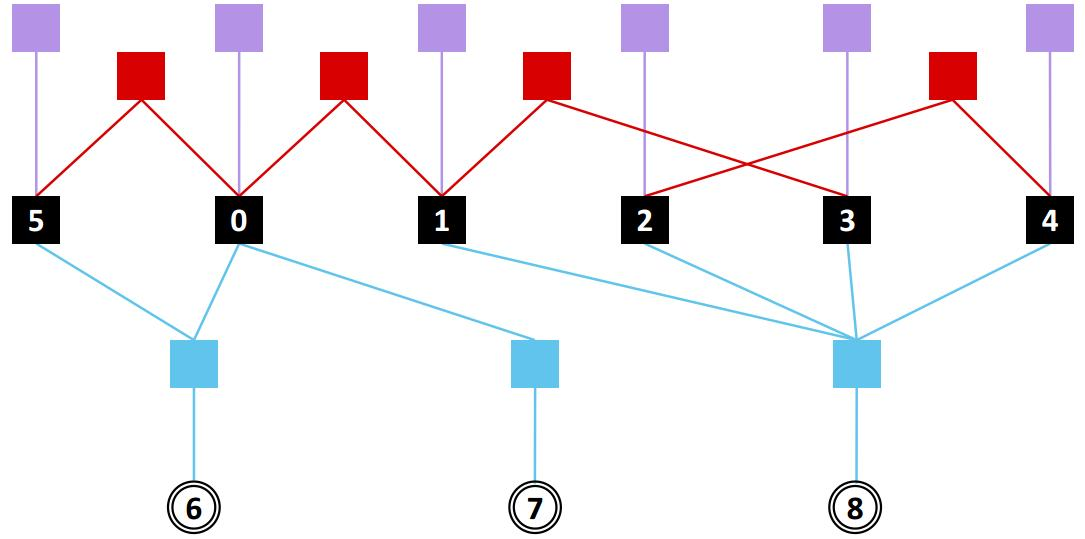
\includegraphics[width=0.9\textwidth]{img/whole-model.pdf}
\caption{ \textbf{我们问题的因子图表示} }
\label{fig:graph}
\end{figure}

\section{有环图的预测}
\label{subsec:inference}

\subsection{因子图表示}
在图\ref{fig:graph}中,我们将问题用因子图去描述。
因为实际上我们的问题是一个图模型问题,变量之间有依赖关系,而因子图就是图模型问题中描述变量之间关系的最好方式。
其中,黑色矩形节点表示人体躯干变量,双环圆形节点表示衣服属性变量,其它颜色的方块表示变量之间的依赖关系。
从因子图\ref{fig:graph}可以看出,我们问题的结构是一个有环图,这样就不能用传统的图画式框架算法进行精确高效的优化预测。
因此在算法\ref{alg:inference},我们提出了一个高效的预测算法,来通过坐标下降的方式来求得近似最优解。
算法\ref{alg:inference}的输入是一个测试样本 $\mathbf{x}$ 和模型参数 $\beta$,输出为人体躯干和衣服属性的局部最优解。
具体来说,在每一步迭代中,当衣服属性变量固定时,问题的结构可以变为一个树结构(无环图),这可以通过动态规划算法\cite{ps2}进行优化。
当人体躯干变量固定时,我们可以通过一个高效的贪心算法来求得局部最优解(详见算法\ref{alg:attr})。

\subsection{最优解估计}
%\subsection{人体躯干的预测}
这一小节,我们来介绍一下人体躯干的预测算法。
之前我们提到过,我们的问题结构是一个有环图,但是当衣服属性变量固定时,我们可以进行一个拆换操作。
具体来说,就是将衣服属性节点作为其相关人体躯干变量节点的子节点,这样就构成一个无环树状图。
因此,我们在传统的图画式结构算法框架上进行了扩展改进,提出一个新的扩展版图画式算法来解决这个有环图问题。
在图\ref{fig:graph}中,我们用不同颜色的节点来表示变量之间的依赖关系分值,
紫色节点代表关于形状的分值,红色节点代表关于形变的分值。
淡绿色的节点代表了我们扩展版图画式算法的主要核心部分,它表示了每个衣服属性变量和其对应的人体躯干之间的依赖关系分值。
因此,我们在算法\ref{alg:ps}中描述了我们的人体躯干预测算法。
我们用符号 $C_i$ 来表示节点 $i$ 的子节点。
在算法\ref{alg:ps}的第3--5行,我们计算了关于形状的分值和衣服属性特征的分值。
在第7行,我们计算出了父子节点之间对应的依赖关系分值。
在第8--12行中,我们采用动态规划计算了节点之间的分值传递过程,每步中父亲节点的分值依赖于所有子节点的分值。
接着在第14--17行中,我们采用了一个自顶向下的方法来找到每一个人体躯干的最优候选解。
通过以上步骤,我们就求得了人体躯干的最优解。

\begin{algorithm}
\caption{人体姿势的预测算法}
\begin{algorithmic}[1]
    \REQUIRE 测试图片样本 $\mathbf{x}$, 模型参数 $\beta$ ,  衣服属性的类别标签值 $\mathbf{a}$
    \ENSURE 人体姿势的最优解 $\mathbf{p^*}$
    \STATE 记人体姿势的最优解集为 $\mathbf{p^*} = \emptyset$
    \STATE 记节点0为根节点
    %\STATE Perform the bottom-up process to compute the score cost for each candidate
    \FOR{ 对于节点 $i$ 的每个候选解 $\mathbf{p}_i$  }
        \STATE 记 $m(\mathbf{p}_i) = \langle \beta_p^i, \phi_p(\mathbf{x}, p_i) \rangle + \langle \beta_{pa}^r, \Psi_{pa}(\mathbf{x}, P_r, a_r) \rangle$
    \ENDFOR
    \FOR{ 对于父亲节点 $j$ 和 $\mathbf{p}_i$ 的子节点 $i$ 的每个候选解 $\mathbf{p}_j$  }
        \STATE set $l(\mathbf{p}_i, \mathbf{p}_j) = \langle \beta_p^{ij}, \psi_p(\mathbf{x}, p_i, p_j) \rangle$
        \IF{ $i$ 是一个叶子节点 }
            \STATE $B_i(\mathbf{p}_j) = \max_{\mathbf{p}_i} (m(\mathbf{p}_i) + l(\mathbf{p}_i, \mathbf{p}_j) )$
        \ELSE
            \STATE $B_i(\mathbf{p}_j) = \max_{\mathbf{p}_i} (m(\mathbf{p}_i) + l(\mathbf{p}_i, \mathbf{p}_j) + \sum_{v \in C_i} B_v(\mathbf{p}_i) )$
        \ENDIF
    \ENDFOR
    %\STATE perform the top-down process to find the best candidate for each human part
    \STATE 为根节点找出最优的解: \\
        $\mathbf{p}_0^* = \arg \max_{\mathbf{p}_0} ( m(\mathbf{p}_0) + \sum_{v \in C_0} B_v(\mathbf{p}_0) )$
    \FOR{ 对于每个父亲-孩子节点对 ($\mathbf{p}_j^*, \mathbf{p}_i$) }
        \STATE $\mathbf{p}_i^* = \arg \max_{\mathbf{p}_i} B_i(\mathbf{p}_j^*)$
    \ENDFOR
\end{algorithmic}
\label{alg:ps}
\end{algorithm}

\section{本章小结}
本章是我们论文最核心的一章,详细描述了本文中提到的基于隐变量衣服属性的人体姿势预测方法。
主要分为三部分,一是联合特征设计,二是模型参数学习,三是有环图预测方法。
联合特征设计是我们算法框架第一步,也是比较关键的一步。
模型参数学习中,我们采用含有隐变量的结构式学习算法,由于包含了隐变量,优化函数变为了非凸函数,
所以不能直接采用梯度下降方法。我们采用迭代式算法来求得近似解。
在预测算法中,我们问题结构变为了有环图,对于无环图我们可以很高效的采用动态规划算法来求得全局最优解,
但是对于有环图,我们无法直接求得全局最优解,于是我们提出了迭代地固定一类变量,来求解另一类变量的局部最优解,
从而求得整个问题的局部最优解。

